\section{Etudes préalables}

\subsection{Présentation du projet}

Ce projet à été mis en place selon notre propre initiative et nous avons donc défini les objectifs à atteindre ainsi que les fonctionnalités de nous même, avec l'aide du tuteur de projet.

Le but de ce projet est de proposer une manière simple pour tout le monde de pouvoir s'orienter dans le locaux de l'ISIMA. Une fois cette solution éprouvée avec les bâtiments de l'ISIMA, nous pouvons penser l'étendre à n'importe quel autre bâtiment donc nous pouvons avoir les plans. Cette idée est inspirée d'un film de Harry Potter, avec la fameuse carte du Maraudeur qui lui permet de suivre les déplacements de tout le monde dans Poudlard.

De manière générale, nous devons être capable de visualiser une carte de l'ISIMA, mais également de pouvoir trouver facilement un bureau ou une salle de cours. De plus, il serait intéréssant de pouvoir également localiser n'importe quelle autre personne visualisant la carte en même temps.
Cette visualisation doit s'actualiser assez rapidement pour que la location de personnes soit la plus précise possible pour les utilisateurs.

\subsection{Analyse de l'existant}

Suivi dans les bâtiments...

\subsection{Spécifications du projet}

Etant donné que peu de solutions sont disponibles sur le marché, nous avons choisi de partir de zéro et créer notre solution.

La solution la plus évidente en terme de support de visualisation pour les utilisateurs et de leur proposer une application qu'ils pourront installer sur leur smartphone, pc, montre connectée ou encore tablette.
Afin de rendre cette application dynamique et de proposer un suivi de position d'utilisateurs en temps réel, il est convenu d'utiliser un Service Web. Ce service permettra également de stocker des informations utiles aux utilisateurs, ce qui permettra également d'alléger le volume de données stockées sur leurs terminaux.

\subsubsection{Architecture}

L'architecture choisie pour organiser notre solution est la suivante.

\begin{figure}[H]
    \centering
    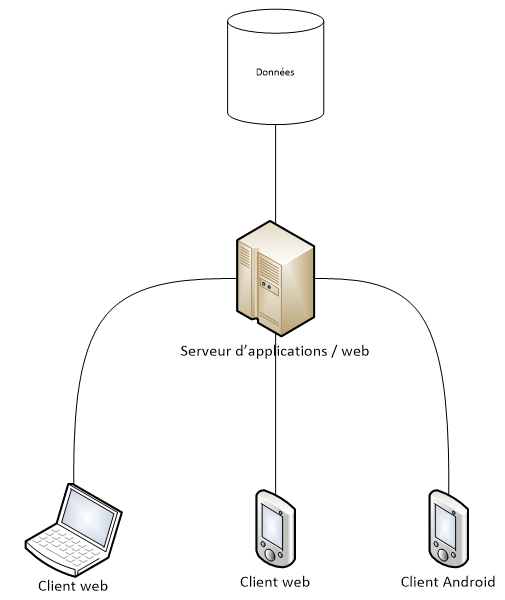
\includegraphics[height=10cm]{../infrastructure.png}
    \caption{Architecture}
    \label{architecture}
\end{figure}

Nous pouvons observer dans la figure~\ref{architecture} que celle-ci ressemble à une architecture client/serveur, ce qui est le but recherché.

\subsubsection{Partie serveur}
La partie centrale est celle du Web Service. Le serveur doit etre capable de répondre aux différentes connexions et requêtes des utilisateurs (se connectant sur l'application Android ou tout autre...). Le serveur sera un service Web permettant (au minimum) :
\begin{itemize}
    \item de s'authentifier
    \item d'obtenir les positions d'autres personnes connectées sur l'application
    \item obtenir la liste des personnes connectées
    \item envoyer la position actuelle de l'utilisateur connecté
    \item proposer l'apk
\end{itemize}

Le serveur pourra aussi en option faire :
\begin{itemize}
    \item historique des positions
    \item calcul d'itinéraire
    \item partage de position
\end{itemize}

Le serveur comportera une base de données dans laquelle les informations des utilisateurs seront stockées (login / mot de passe). Les dernières positions des utilisateurs seront également stockées. Il y aura une table permettant d'identifier quels utilisateurs sont actuellement actifs.
Il a été convenu d'utiliser NodeJS du coté serveur pour plusieurs raisons :
\begin{itemize}
    \item rapidité de mise en place
    \item faible nombre d'utilisateurs
    \item l'un de nous a des connaissances dessus
\end{itemize}

Base de données
La base de données utilisée est une base MongoDB. Ce type de base de données est trés simple à mettre en place et se base sur un format JSON binaire pour stocker les différentes informations que nous souhaitons. Ceci va faire qu'il est facile d'utiliser les résultats des requêtes directement en Javascript.
Requetes sur le web service
Des URL sont mises à disposition par le service et permettent d'effectuer certaines tâches. Le passage de paramètres pour ces URL se fait directement dans le corps de la requête sous forme de JSON.
Les réponses du service sont sous forme d'objet JSON dans le corps de la réponse. Les réponses contiennent les champs suivants :

\lstset{language=Javascript}
\begin{lstlisting}[caption=Corps de la réponse serveur]
{
    'status': 'ok' / 'fail', // L'état de la requête
    'error': 'description' // Une description de l'erreur s'il y en a une
}
\end{lstlisting}


La plupart des requêtes décrites nécéssitent que l'utilisateur soit authentifié.
/login
La première requête à effectuer sur le service doit s'effectuer avec la méthode POST sur cette URL. Pour se connecter, l'utilisateur doit envoyer les paramètres suivants: 
\lstset{language=Javascript}
\begin{lstlisting}[caption=Corps de la requête login]
{
    'name': 'username', // Le nom de l'utilisateur à connecter
    'location': [1.0, 2.0, 3.0] // La position courrante de l'utilisateur
}
\end{lstlisting}

/who
Cette URL permet de récupérer en méthode GET une liste de noms de personnes actuellement en ligne. Le retour est sous la forme suivante:
\lstset{language=Javascript}
\begin{lstlisting}[caption=Corps de la requête who]
{
    'list': [
        'userName1',
        'userName2',
        'userName3'
    ]
}
\end{lstlisting}

/where
En utilisant la méthode GET, cette URL retourne la liste des utilisateurs ainsi que leur position. En utilisant la méthode POST et en passant les paramètres adéquats, l'utilisateur peut mettre à jour sa position.
En méthode GET, le service renvoie une liste des utilisateurs connectés avec leurs positions :
\lstset{language=Javascript}
\begin{lstlisting}[caption=Corps de la requête where GET]
{
    'list': [
        {
            'name': 'username1',
            'location': [1.0, 2.0, 3.0]
        },
        {
            'name': 'username2',
            'location': [1.0, 2.0, 3.0]
        },
        {
            'name': 'username3',
            'location': [1.0, 2.0, 3.0]
        }
    ]
}
\end{lstlisting}

En utilisant la méthode POST, l'utilisateur met à jour sa position. Les paramètres à envoyer sont les suivants :

\lstset{language=Javascript}
\begin{lstlisting}[caption=Corps de la requête where POST]
{
    'name': 'username',
    'location': [1.0, 2.0, 3.0]
}
\end{lstlisting}

Si l'utilisateur n'est pas connecté au moment de mettre à jour sa position, le serveur va tenter de l'authentifier et sauvegarder sa position.
Partie administration
Les fonctionnalités minimales pour l'application d'administration sont :
\begin{itemize}
    \item visualisation des logs du serveur
    \item visualisation du contenu de la base de donnée
\end{itemize}

Ensuite les fonctionnalités avancées pourront être :
\begin{itemize}
    \item gestion des utilisateurs
\end{itemize}


\subsubsection{Partie Android}
Une seconde partie comporte une application Android (qui pourrait être déclinée pour iOS et Windows Phone). Cette application permettra :
\begin{itemize}
    \item de s'inscrire
    \item de se connecter
    \item envoyer sa position gps au service web
    \item recevoir les positions gps d'autres utilisateurs connectés
    \item visualiser en temps réel sur une carte les positions
\end{itemize}

L'application pourra évoluer et proposer :
\begin{itemize}
    \item la carte en version 3D
    \item la carte en version VR
    \item l'ajout d'informations sur la carte (lieu / point de rdv)
\end{itemize}

Le choix d'une application Android se justifie par :
\begin{itemize}
    \item la communauté Android est active
    \item la quantité de terminaux
    \item l'un de nous a des connaissances en Android
\end{itemize}
La mise à jour des positions est soit faite par l'application qui effectue une requête sur le serveur, soit c'est le serveur qui renvoie les positions des utilisateurs ayant bougé d'un delta suffisant qui permet sa mise à jour chez les utilisateurs. Les frameworks 3.X+ seront supportés pour fonctionner sur un maximum de terminaux.


\subsubsection{Intégration continue}
Un des objectifs de ce projet est de mettre en place une intégration continue et un déploiement automatique. Pour ce faire il est nécessaire d'avoir deux serveurs :
\begin{itemize}
    \item un serveur d'application
    \item un serveur d'intégration
\end{itemize}

Le premier sera certainement un CaaS Amazon pour NodeJS. Le serveur d'intégration sera un serveur Travis CI puisqu'il gère à la fois le NodeJS et l'Android (nouvelle fonctionnalité). Cela permettra contrairement à un serveur Jenkins de déployer facilement sans avoir à gérer un serveur mais juste en utilisant un service.

\subsection{Organisation du travail}

L'organisation temporelle théorique du travail est décrite dans le diagramme de Gantt ci-dessous.

\begin{landscape}
    \begin{figure}[h]
        \centering
        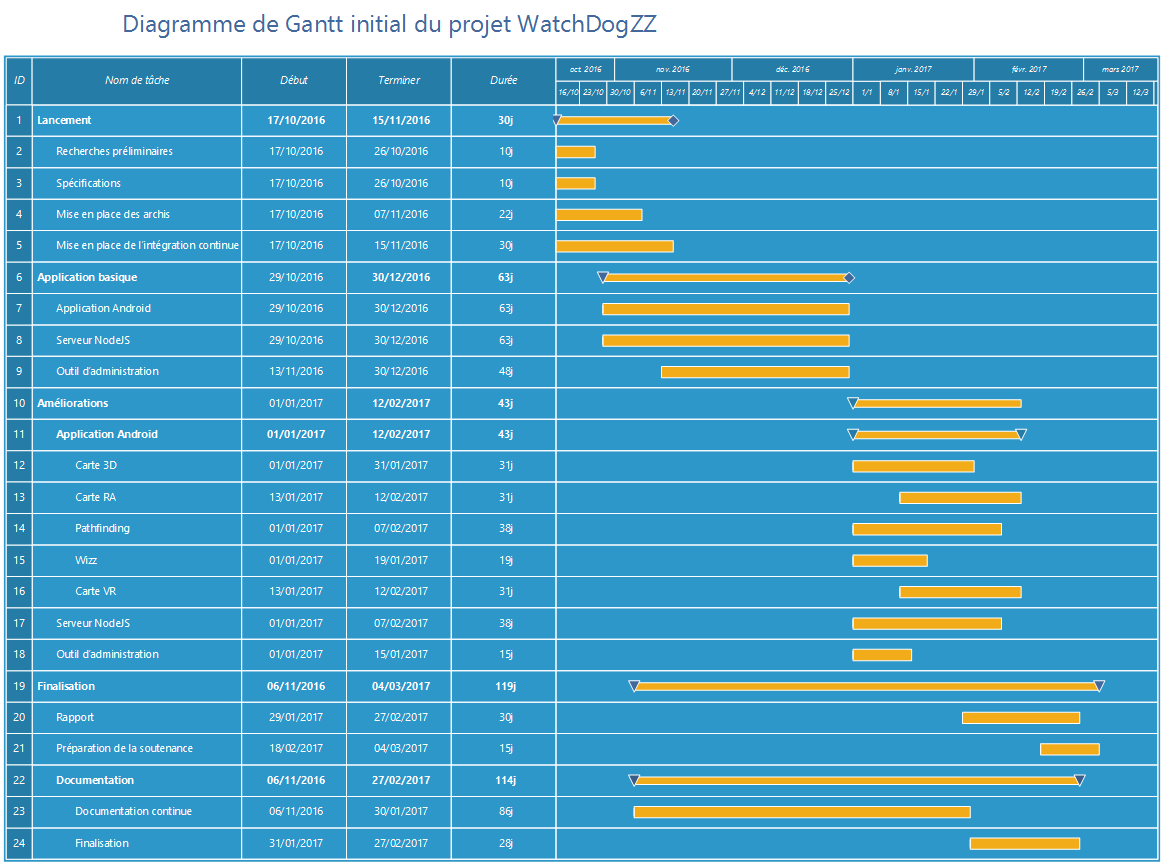
\includegraphics[height=\textwidth]{../gantt_initial.png}
        \caption{Diagramme de Gantt théorique}
    \end{figure}
\end{landscape}

suite...